\documentclass[a4paper]{article}
\usepackage[english]{babel}
\usepackage[utf8]{inputenc}
\usepackage[left=3.0cm, right=3.0cm]{geometry}
\usepackage{amsmath}
\usepackage{graphicx}
\usepackage{fancyhdr}
\usepackage{hyperref}
\usepackage{enumerate}
\usepackage{amssymb}
\usepackage{amsthm}
\usepackage{tikz-cd}
\usepackage{ytableau}

\newcommand{\R}{\mathbb{R}}
\newcommand{\Z}{\mathbb{Z}}
\newcommand{\N}{\mathbb{N}}
\newcommand{\C}{\mathbb{C}}
\newcommand{\Q}{\mathbb{Q}}
\newcommand{\F}{\mathbb{F}}
\newcommand{\E}{\mathbb{E}}
\renewcommand{\P}{\mathbb{P}}
\newcommand{\f}[1]{\text{#1}}
\newcommand{\<}{\langle}
\renewcommand{\>}{\rangle}
\renewcommand{\^}{\wedge}
\renewcommand{\v}{\vee}


\pagestyle{fancy}
\fancyhf{}
\lhead{\today}
\chead{MATH H113}
\rhead{Albert Zhang}
\cfoot{\thepage}

\makeatletter
\renewcommand{\@seccntformat}[1]{}
\makeatother

% \setcounter{secnumdepth}{0}
\setlength{\parindent}{0pt}
\setlength{\parskip}{8pt}

\title{\textbf{H113 --- ABSTRACT ALGEBRA}}
\author{\large Taught by A. Givental \\
Notes \& Exercises by Albert Zhang}
\date{Spring 2019}

\begin{document}

\maketitle
\tableofcontents
\newpage

%%%%%%%%%%%%%%%%%%%% 
\section{Preliminary Notions}
\subsection{Homework 1}
\begin{enumerate}
    \item \textbf{Solution:}
    (fails reflexivity) First consider the set $\{T, F\}$ of the two true and false boolean values. If we use logical \textbf{and} (\&) as our binary relation, we see that:
    \begin{itemize}
        \item Reflexivity: is not satisfied, as F\&F is not true.
        \item Symmetry: is satisfied. The only case we have to consider is T\&T, and switching the operands gives the same relation, which is still true.
        \item Transitivity: is satisfied. The only situation we have to consider is if T\&T and T\&T. But then T\&T is trivial.
    \end{itemize}
    
    (fails symmetry) Consider the set $\Z$ with the binary operation $|$, or "divides". Then we have:
    \begin{itemize}
        \item Reflexivity: is satisfied. Any integer divides itself.
        \item Symmetry: is not satisfied. E.g. $4 | 8$ but $8 \nmid 4$.
        \item Transitivity: is satisfied. If $a \mid b$ and $b \mid c$, then we can write $c = mb$ and $b = na$ for integers $m$ and $n$. It follows then that $c = mna$, and thus $a \mid c$.
    \end{itemize}
    
    (fails transitivity) Consider the set of vectors in $\R^2$. Define a binary relation $\approx$ on $\R^2$ as $x \approx y$ if $|x - y| \leq 1$, or in other words, $x \approx y$ if the distance between the two points is less than or equal to 1. Then clearly for every $x, y \in \R^2$, $x \approx x$, and if $x \approx y$ then $y \approx x$. However, consider the points $(-1, 0)$, $(0, 0)$, and $(1, 0)$. We have that $(-1, 0) \approx (0, 0)$ and $(0, 0) \approx (1, 0)$ but $(-1, 0) \not\approx (1, 0)$.
    
    \item \textbf{Solution:}
    We keep track of the coefficients as we repeatedly apply the Euclidean:
    \begin{align*}
        1 * 1763 - 1 * 991 &= 772 \\
        -1 * 1763 + 2 * 991 &= 219 \\
        4 * 1763 - 7 * 991 &= 115 \\
        -5 * 1763 + 9 * 991 &= 104 \\
        9 * 1763 - 16 * 991 &= 11 \\
        -86 * 1763 + 153 * 991 &= 5 \\
        181 * 1763 - 322 * 991 &= 1.
    \end{align*}
    It follows that 1763 and 991 are relatively prime. That is, $d = (1763, 991) = 1 = 181 * 1763 - 322 * 991$. In mod  1763, we have
    \begin{align*}
        181 * 1763 - 322 * 991 &\equiv 1 \f{(mod 1763)} \\
        (-322) * 991 &\equiv 1 \f{(mod 1763)} \\
        1441 * 991 &\equiv 1 \f{(mod 1763)}.
    \end{align*}
    Thus 991 is invertible, with inverse 1441 in mod 1763.
    
    \item \textbf{Solution:}
    Consider the Norm function $N: R \to \Z$ given by $a + b\sqrt{-5} \mapsto a^2 + 5b^2$ for $a, b \in \Z$. We know that $N$ is multiplicative, that is 
    \begin{align*}
        N((a + b\sqrt{-5})(c + d\sqrt{-5})) &= N((ac - 5bd) + (ad + bc)\sqrt{-5}) \\
        &= a^2c^2 + 25b^2d^2 + 5a^2d^2 + 5b^2c^2 \\
        &= (a^2 + 5b^2)(c^2 + 5d^2) \\
        &= N(a + b\sqrt{-5})N(c + d\sqrt{-5}).
    \end{align*}
    Now, suppose we have $2 = zw$ for $z, w \in R$. Then taking the norm of both sides, we get
    \begin{align*}
        4 &= N(2) \\
            &= N(zw) \\
            &= N(z)N(w),
    \end{align*}
    and since the codomain of $N$ is $\Z$, we get that the product $N(z)N(w)$ must either be $(\pm 2)(\pm 2)$, $(\pm 4)(\pm 1)$, or $(\pm 1)(\pm 4)$. Since the norm of any element of $R$ must be of the form $a^2 + 5b^2$, $a, b \in \Z$, the only possible values of $z$ is $\pm 1$ and $\pm 2$. It follows that 2 is irreducible in $R$. Now, to show 2 is not prime in $R$, consider
    \begin{align}
        2 * 3 = 6 = (1 + \sqrt{5}i)(1 - \sqrt{5}i).
    \end{align}
    We see that $2 \mid (1 + \sqrt{5}i)(1 - \sqrt{5}i)$, but clearly $2 \nmid (1 + \sqrt{5}i)$ and $2 \nmid (1 - \sqrt{5}i)$. Thus 2 is not prime.
    
    Similarly, suppose $3 = zw$ for some $z, w \in R$. Then we get $9 = N(3) = N(zw) = N(z)N(w)$, and by similar logic as above, we obtain that $N(z)N(w)$ must be $(\pm 9)(\pm 1)$ or $(\pm 1)(\pm 9)$, which implies that $z = \pm 1, \pm 3$, and 3 is irreducible in $R$. Further by (1), we get $3 \mid (1 + \sqrt{5}i)(1 - \sqrt{5}i)$ but clearly $3 \nmid (1 + \sqrt{5}i)$ and $3 \nmid (1 - \sqrt{5}i$.
    
    Thus, 2 and 3 are irreducible but both are not prime in $R$.
    
    
    \item First, we find the 4 permutations of $X$ that induce the identity permutation on $Y$. In order for the ordering of $(VHS)$ to remain the same, the vertical partition must still be $AB$ and $CD$, the horizontal partition must still be $BC$ and $AD$, and the diagonal partition must still be $AC$ and $BD$. It is easy to verify that the only four such permutations of $X$ are:
    \begin{align*}
        I_0: &\quad (ABCD) &\quad \f{(identity)}\\
        I_1: &\quad (AC)(BD) &\quad (180^\circ \f{ rotation)}\\
        I_2: &\quad (AB)(CD) &\quad \f{(vertical reflection)} \\
        I_3: &\quad (AD)(BC) &\quad \f{(horizontal reflection)}
    \end{align*}
    Now, given two permutations $\sigma_X$ and $\tau_X$ of $X$, let $\sigma_Y$ and $\tau_Y$ be their induced permutations on $Y$, respectively. It is clear that $\sigma_Y = \tau_Y$ whenever $\sigma_X = I_k\tau_X$ for some $k \in \{0, 1, 2, 3\}$. We will show that this induces an equivalence relation on the set of permutations $A(X)$ of $X$, and hence produces a one to one correspondence between each of the 6 permutations of $Y$ and equivalence classes of 4 permutations in $X$. For $\sigma, \tau \in A(X)$, say $\sigma \sim \tau$ if for some $k \in \{0, 1, 2, 3\}$, we have that $\sigma = I_k\tau$. We now verify:
    \begin{itemize}
        \item (reflexivity) Clearly each permutation is just the product of itself and the identity permutation $I_0 = (ABCD)$. i.e. $\sigma = I_0\sigma$ for every $\sigma \in A(X)$.
        \item (symmetry) Note that $I_0$ and $I_1$ are their own inverses, respectively, and $I_2$ and $I_3$ are inverses of each other. It follows that if $\sigma, \tau \in A(X)$ and $\sigma \sim \tau$, or $\sigma = I_k\tau$, we can multiply by the inverse to obtain $\tau = I_k^{-1}\sigma$, or $\tau \sim \sigma$.
        \item (transitivity) This follows from the fact that composition of any two identity permutations in $\{I_0, I_1, I_2, I_3\}$ results in another identity permutation among the same set. In particular, $I_k^2 = I_0$ and $I_0I_k = I_kI_0 = I_k$ for every $k$, $I_1I_2 = I_2I_1 = I_3$, $I_1I_3 = I_3I_1 = I_2$, and $I_2I_3 = I_3I_2 = I_1$.
    \end{itemize}
    
    Now, each of the 6 permutations of $Y$ are in one to one correspondence to an equivalence class in $X$ consisting of exactly 4 permutations differing from each other only by some composition of the 4 identity permutations.
    
\end{enumerate}
\section{Homework 2}

\begin{enumerate}
    \item \textbf{Packet Routing}
    
    (a) Let $S$ be the random variable counting the number of arriving packets in the time interval $[0, 1]$, and let $X$ be the random variable counting the number of packets routed to $A$. We will show that $X$ is poisson distributed with parameter $\lambda p$. We compute the probability that $X = k$ as a summation based on the number of packets that arrive at the switch:
    \begin{align*}
        \P[X = k] &= \sum\limits_{i = k}^\infty \P[S = i]\binom{i}{k}(1 - p)^{i - k}p^k \\
            &= \sum\limits_{i = k}^\infty \frac{e^{-\lambda}\lambda^i}{i!}\binom{i}{k}(1 - p)^{i - k}p^k \\
            &= \frac{\lambda^k p^k e^{-\lambda}}{k!}\sum\limits_{j = 0}^\infty \frac{\lambda^j(1 - p)^j}{j!} \\
            &= \frac{\lambda^k p^k e^{-\lambda}e^{\lambda(1 - p)}}{k!} \\
            &= \frac{e^{-\lambda p}(\lambda p)^k}{k!} \sim \f{Poisson}(\lambda p).
    \end{align*}
    
    (b) Consider $\P[A = k | B = 0]$. This is equal to $\P[S = k]p^k = e^{-\lambda}\frac{\lambda^k}{k!}p^k$, that is, the probability that $k$ packets arrive at the switch and all $k$ of these packets are routed to $A$. However, by our result from part (a), $\P[A = k] = e^{-\lambda p}\frac{(\lambda p)^k}{k!}$. Thus, the number of packets routed to $A$ and the to $B$ cannot be independent since
    \[
    \P[A = k | B = 0] = e^{-\lambda}\frac{\lambda^k}{k!}p^k \neq e^{-\lambda p}\frac{(\lambda p)^k}{k!} = \P[A = k].
    \]
    
    \item \textbf{Compact Arrays}
    
    Note that $X = i - (\f{\# of 0's that appear before ith index})$. We can separate the second portion into i.i.d. indicator random variables $I_1, \dots, I_{i - 1}$, where $I_k$ indicates whether a 0 appears in the $k$th position or not. Then we have that
    \begin{align*}
    \E[X] &= \E[i - (\f{\# of 0's that appear before ith index})] \\
        &= i - \E[I_1 + \dots + I_{i - 1}] \\
        &= i - (i - 1)\E[I_1] \\
        &= i - (i - 1)\frac{1}{10} \\
        &= \frac{9i + 1}{10}.
    \end{align*}
    Now, we calculate the variance, using the same indicator variables and the property that they are mutually independent and identically distributed:
    \begin{align*}
        \f{Var}(X) &= \f{Var}(i - (I_1 + \dots + I_{i - 1})) \\
            &= \f{Var}(I_1 + \dots + I_{i - 1}) \\
            &= \f{Var}(I_1) + \dots + \f{Var}(I_{i - 1}) \\
            &= (i - 1)(\E[I_1^2] - \E[I_1]^2) \\
            &= (i - 1)(\frac{1}{10} - \frac{1}{100}) \\
            &= \frac{9i - 9}{100}.
    \end{align*}
    
    \item \textbf{Message Segmentation}
    
    (a) First, we note that the support of our PMF $f$ is $(q, r)$ where $0 \leq r < m$ whenever $q > 0$ and $0 < r < m$ whenever $q = 0$ (since $N$ is strictly positive and $N = mq + r$) for integers $q$ and $r$. Let $N$ be the random variable of number of bytes in the message. Now, we find our PMF to be
    \begin{align*}
        f(q, r) &= \P[Q = q, R = r] \\
            &= \P[N = mq + r] \\
            &= (1 - p)^{mq + r - 1}p
    \end{align*}
    where $q$ and $r$ are restricted to the support mentioned above.
    
    (b) First, we compute the marginal PMF of $Q$ when $q > 0$:
    \begin{align*}
        \P[Q = q] &= \sum\limits_{i = 0}^{m - 1}\P[Q = q, R = i] \\
            &= \sum\limits_{i = 0}^{m - 1}(1 - p)^{mq + i - 1}p \\
            &= (1 - p)^{mq - 1}p\sum\limits_{i = 0}^{m - 1}(1 - p)^i \\
            &= (1 - p)^{mq - 1}p\left(\frac{1 - (1 - p)^m}{1 - (1 - p)}\right) \\
            &= (1 - p)^{mq - 1} - (1 - p)^{mq + m - 1}.
    \end{align*}
    Now, if $q = 0$, then we replace the starting index 0 with 1 and instead get:
    \begin{align*}
        \P[Q = 0] &= \sum\limits_{i = 1}^{m - 1}\P[Q = 0, R = i] \\
            &= \sum\limits_{i = 1}^{m - 1}(1 - p)^{i - 1}p \\
            &=p\left(\frac{1 - (1 - p)^{m - 1}}{1 - (1 - p)}\right) \\
            &= 1 - (1 - p)^{m - 1}
    \end{align*}
    
    On the other hand, we compute the marginal PMF of $R$ for $R = r > 0$:
    \begin{align*}
        \P[R = r] &= \sum\limits_{i = 0}^\infty \P[Q = i, R = r] \\
            &= \sum\limits_{i = 0}^\infty(1 - p)^{mi + r - 1}p \\ 
            &= (1 - p)^{r - 1}p\sum\limits_{i = 0}^\infty((1 - p)^m)^i \\
            &= \frac{p(1 - p)^{r - 1}}{1 - (1 - p)^m}
    \end{align*}
    
    Now, we compute the marginal PMF of $R$ when $R = 0$:
    \begin{align*}
        \P[R = 0] &= \sum\limits_{i = 1}^\infty \P[Q = i, R = 0] \\
            &= \sum\limits_{i = 1}^\infty(1 - p)^{mi - 1}p \\
            &= \frac{p}{1 - p}\left(\frac{(1 - p)^m}{1 - (1 - p)^m}\right) \\
            &= \frac{p(1 - p)^{m - 1}}{1 - (1 - p)^m}.
    \end{align*}
    
    (c) Now that we are given $N > m$, $q$ is at least 1, and our support becomes nicer and with less casework. That is, our support now consists of points $(q, r)$ for integers $q$ and $r$ that satisfy $q > 0$ and $0 \leq r < m$.
    
    The marginal PMF of $Q$ stays the same:
     \begin{align*}
        \P[Q = q] &= \sum\limits_{i = 0}^{m - 1}\P[Q = q, R = i] \\
            &= (1 - p)^{mq - 1} - (1 - p)^{mq + m - 1}.
    \end{align*}
    
    We compute the updated marginal PMF of $R$:
    \begin{align*}
        \P[R = r] &= \sum\limits_{i = 1}^\infty\P[Q = i, R = r] \\
        &= \sum\limits_{i = 1}^\infty(1 - p)^{mi + r - 1}p \\
        &= p(1-p)^{m + r - 1}\sum\limits_{i = 0}^\infty(1 - p)^{mi} \\
        &= \frac{p(1 - p)^{m + r - 1}}{1 - (1 - p)^m}.
    \end{align*}
    
    \item \textbf{Almost Fixed Points of a Permutation}
    
    We can split $X$ into indicator variables $I_1, \dots, I_n$ where $I_k$ indicates whether or not $k$ is almost a fixed point of a given permutation. Then since the probability of a number being almost a fixed point is just $\frac{3}{n}$ (3 possible "almost fixed points", the two adjacent points and itself), we get the expectation using linearity
    \begin{align*}
        \E[X] &= \E[I_1 + \dots + I_n] \\
            &= \E[I_1] + \dots + \E[I_n] \\
            &= n \cdot \frac{3}{n} \\
            &= 3.
    \end{align*}
    
    For variance, we must split our calculations into cases with respect to $n$.
    
    Case 1 ($n = 1$):
    The only permutation sends 1 to 1. Thus the variance is 0.
    
    Case 2 ($n = 2$):
    There are two permutations, both of which produce 2 almost fixed points. Thus the variance is 0 again.
    
    Case 3 ($n = 3$):
    There are six permutations, all of which produce 3 almost fixed points. Thus the variance is 0 again.
    
    Case 4: ($n = 4$):
    Look at case 5 first. The only changes we need to make are to the counting of $\sum_{k \neq j}\E[I_kI_j]$. First, if $k$ and $j$ are adjacent, the expectation stays the same, namely
    \[
        \frac{14}{n - 1} = \frac{14}{3}.
    \]
    Now, there are 4 ways such that $k$ and $j$ are two indices apart. WLOG consider points 1, 2, 3, 4, where $k = 1, j = 3$. Then there are 7 ways to assign an ordered pair so that 1 and 3 are almost fixed points: (1, 2), (1, 3), (1, 4), (2, 3), (2, 4), (4, 2), (4, 3). So the expectation for this case is 
    \[
        4 \cdot \frac{7}{n(n - 1)} = \frac{7}{3}.
    \]
    Adding everything up, we get
    \begin{align*}
        \f{Var}(X) &= \frac{14}{3} + \frac{7}{3} - 6 \\
            &= 1.
    \end{align*}
    
    
    Case 5 ($n > 4$): 
    We split our random variable $X$ into indicators $I_1, \dots, I_n$ where $I_k$ indicates whether or not $k$ is an almost fixed point. Then we can use linearity to get
    \begin{align*}
        \f{Var}(X) &= \E[X^2] - \E[X]^2 \\
            &= \E[(I_1 + \dots + I_n)^2] - 3^2 \\
            &= \E[(I_1^2 + \dots + I_n^2) + \sum_{k \neq j}I_kI_j] - 9 \\
            &= \sum_{i = 1}^n\E[I_i^2] + \sum_{k \neq j}\E[I_kI_j] - 9 \\
            &= n\left(\frac{3}{n}\right) + \sum_{k \neq j}\E[I_kI_j] - 9 \\
            &= \left(\sum_{k \neq j}\E[I_kI_j]\right) - 6.
    \end{align*}
    Now, to compute the expectations in the large parentheses, we must account for cases where $k$ and $j$ differ by: one index, two indices, more than two indices.
    
    (one index) There are $2n$ ways to choose $k$ and $j$ to produce this case. WLOG consider the four points 1, 2, 3, 4, where $j = 2, k = 3$. Then corresponding to points 2 and 3 we can assign 7 possible ordered pairs such that both are almost fixed points: (1, 2), (1, 3), (1, 4), (2, 3), (2, 4), (3, 2), (3, 4). Since there are $n(n-1)$ ways to assign any ordered pair, we have a probability of $\frac{7}{n(n-1)}$ for this case. Furthermore, the total expectation in this case would amount to
    \[
        2n \cdot \frac{7}{n(n-1)} = \frac{14}{n-1}.
    \]
    
    (two indices) Once again, there are $2n$ ways to choose $k$ and $j$ to produce this case. WLOG consider the five points 1, 2, 3, 4, 5, where $j = 2, k = 4$. Then corresponding to points 2 and 4 we can assign 8 possible ordered pairs such that both are almost fixed points: (1, 3), (1, 4), (1, 5), (2, 3), (2, 4), (2, 5), (3, 4), (3, 5). Similar to the previous case, the total expectation in this case would amount to
    \[
        2n \cdot \frac{8}{n(n-1)} = \frac{16}{n-1}.
    \]
    
    (more than two indices) Since there are $n(n-1)$ ways to pick any ordered pair of points, we subtract the previous two cases to get $n(n-1) - 4n = n^2 - 5n$ ways to choose $k$ and $j$ to produce this case. Since there is no interference between the two points, there would be $3\cdot3 = 9$ ways to assign almost fixed points. Therefore, the total expectation in this case would amount to
    \[
        (n^2 - 5n)\frac{9}{n(n-1)} = \frac{9n - 45}{n - 1}.
    \]
    
    Summing this all together, we get
    \begin{align*}
        \f{Var}(X) &= \frac{14}{n - 1} + \frac{16}{n - 1} + \frac{9n - 45}{n - 1} - 6 \\
            &= \frac{3n - 9}{n - 1} = 3 - \frac{6}{n - 1}.
    \end{align*}
    
    Now, noticing that the answers to case 3 and 4 satisfy the formula derived in case 5, we summarize:
    \[
    \f{Var}(X) = \begin{cases}
        0 & \f{ for } n = 1, 2, \\
        3 - \frac{6}{n - 1} & \f{ for } n > 2.
    \end{cases}
    \]
    
    \item \textbf{Introduction to Information Theory}
    
    (a) Using the definition, we have
    \begin{align*}
        H(X) &= -\sum_x p(x)\log p(x) \\
            &= -\sum_x \log \left(p(x)^{p(x)}\right) \\
            &= -\left(\log\left(\prod_x p(x)^{p(x)}\right)\right) \\
            &\geq 0,
    \end{align*}
    since the $0 \leq p(x) \leq 1$ for all $x$, and we have a product of terms between 0 and 1, of which the log will return a nonpositive real value, and negating gives us a nonnegative real value.
    
    (b) If $p = 1$ or $p = 0$, then the entropy would be 0. So intuitively, $p = 1/2$ should have a higher entropy than $p = 1/3$.
    
    For $p = 1/2$, we have
    \begin{align*}
        H(X) &= -\sum_{k = 0}^1 \frac{1}{2}\log_2\frac{1}{2} \\
            &= -\left(-\frac{1}{2} - \frac{1}{2}\right) \\
            &= 1.
    \end{align*}
    
    For $p = 1/3$, we have
    \begin{align*}
        H(X) &= -\left(\frac{1}{3}\log_2\frac{1}{3} + \frac{2}{3}\log_2\frac{2}{3}\right) \\
            &= -\left(\log_2\left(\left(\frac{1}{3}\right)^{\frac{1}{3}}\left(\frac{2}{3}\right)^{\frac{2}{3}}\right)\right) \\
            &= -\left(\log_2\left(\left(\frac{4}{27}\right)^{\frac{1}{3}}\right)\right) \\
            &\approx 0.9183...
    \end{align*}
    
    So the entropy when $p = 1/2$ is higher.
    
    (c) First, we see that
    \begin{align*}
        \P[Y = 0] &= \frac{1}{2}(1 - p_e) \\
        \P[Y = ~?] &= \frac{1}{2}(p_e) + \frac{1}{2}(p_e) = p_e \\
        \P[Y = 1] &= \frac{1}{2}(1 - p_e).
    \end{align*}
    
    Now, we compute the entropy, combining the cases where $Y = 0$ and $Y = 1$:
    \begin{align*}
        H(Y) &= -\left((1 - p_e)\log_2\left(\frac{1}{2}(1 - p_e)\right) + p_e\log_2p_e\right) \\
            &= -\left((1 - p_e)(-1 + \log_2(1 - p_e)) + \log_2\left(p_e^{p_e}\right)\right) \\
            &= 1 - p_e - \log_2\left((1 - p_e)^{1 - p_e}p_e^{p_e}\right).
    \end{align*}
    
    (d) First, we compute the probabilities at each point:
    \begin{align*}
        p(0, 0) &= \frac{1}{2}(1 - p_e) \\
        p(0, ?) &= \frac{1}{2}p_e \\
        p(1, 1) &= \frac{1}{2}(1 - p_e) \\
        p(1, ?) &= \frac{1}{2}p_e.
    \end{align*}
    
    Now, we compute the entropy, combining symmetric cases from above:
    \begin{align*}
        H(X, Y) &= -\left((1 - p_e)\log_2\left(\frac{1}{2}(1 - p_e)\right) + p_e\log_2\left(\frac{1}{2}p_e\right)\right) \\
            &= -\left((1 - p_e)(-1 + \log_2(1 - p_e)) + p_e(-1 + \log_2p_e)\right) \\
            &= 1 - \log_2\left((1 - p_e)^{1 - p_e}p_e^{p_e}\right).
    \end{align*}
    
    \item \textbf{Soliton Distribution}
    
    (a) The probability that a given degree $d$ packet is connected to the chunk we are about to peel off is
    \[
        \frac{\binom{N - k - 1}{d - 1}}{\binom{N - k}{d}} = \frac{\frac{(N - k - 1)!}{(d - 1)!(N - k - d)!}}{\frac{(N - k)!}{d!(N - k - d)!}} = \frac{d}{N - k}.
    \]
    Therefore, using linearity of expectation, the expected number of degree $d$ packets whose degrees will be reduced by one after removing the $(k + 1)$st packet should be 
    \[
    f_k(d) \cdot \frac{d}{N - k}.
    \]
    
    (b) For the $d = 1$ case, we have the following recurrence relation,
    \[
        f_{k + 1}(1) = f_k(2) \cdot \frac{2}{N - k},
    \]
    and if we plug in our desired $f_{k + 1}(1) = 1$ and formula $f_k(d) = (N - k)/[d(d - 1)]$, we see that the above recurrence relation holds:
    \[
        f_{k + 1}(1) = 1 = \frac{N - k}{2(1)} \cdot \frac{2}{N - k} = f_k(2) \cdot \frac{2}{N - k}.
    \]
    
    Now, for the general case where $d = 2,\dots,N$, we have the following recurrence relation,
    \[
        f_{k + 1}(d) = f_k(d + 1)\cdot\frac{d + 1}{N - k} + f_k(d)\cdot\left(1 - \frac{d}{N - k}\right),
    \]
    and if we plug in the formula $f_k(d) = (N - k)/[d(d - 1)]$, once again we see that the recurrence relation holds:
    \begin{align*}
        f_k(d + 1)\cdot\frac{d + 1}{N - k} + f_k(d)\cdot\left(1 - \frac{d}{N - k}\right) &= \frac{N - k}{d(d + 1)}\cdot\frac{d + 1}{N - k} + \frac{N - k}{d(d - 1)}\cdot\frac{N - k - d}{N - k} \\
            &= \frac{1}{d} + \frac{N - k - d}{d(d - 1)} \\
            &= \frac{N - (k + 1)}{d(d - 1)} \\
            &= f_{k + 1}(d),
    \end{align*}
    which is what we wanted. It follows that in order for $f_k(1) = 1$ to hold for $k = 0,\dots,N - 1$, we must have $f_k(d) = (N - k)/[d(d - 1)]$ for all $d = 2,\dots,N$.
    
    From this, we may deduce what $p(d)$ is for each $d > 1$. The probability of $p(d)$ for $d > 1$ satisfies $f_0(d) = N \cdot p(d)$. From the formula above, this gives us that $p(d) = \frac{1}{d(d-1)}$ for $d > 1$. For $d = 1$, we have $1 = f_1(1) = N \cdot p(1)$, which gives us $p(1) = \frac{1}{N}$.
    
    (c) We compute the expectation of $p(\cdot)$:
    \begin{align*}
        \E[p(\cdot)] &= \sum_{i = 1}^n d \cdot p(d) \\
            &= \frac{1}{n} + \sum_{i = 2}^n d \cdot \frac{1}{d(d-1)} \\
            &= \frac{1}{n} + \sum_{i = 2}^n \frac{1}{d - 1} \\
            &= \sum_{i = 1}^{n - 1}\frac{1}{i} \\
            &\approx \ln (n - 1),
    \end{align*}
    or just $\ln n$ for large $n$.
    
\end{enumerate}
\section{Homework 3}

\subsection{Graphical Density}
(a) We have
\[
2\cdot1\cdot A + 1\cdot1\cdot (2A) + 2\cdot1\cdot A = 1,
\]
so $A = \frac{1}{6}$. Below we sketch the p.d.f.'s for $f_X$, $f_Y$, and $f_{X|X+Y\leq3}$, respecitvely:

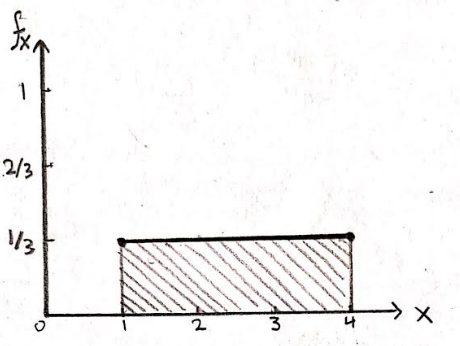
\includegraphics[scale=0.3]{f_X}
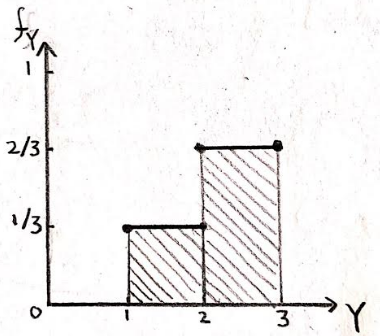
\includegraphics[scale=0.3]{f_Y}
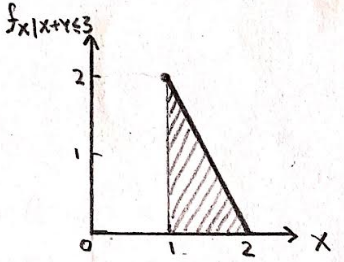
\includegraphics[scale=0.4]{f_conditional}

(b) For $\E[X|Y = y]$, we have symmetry on both $[1, 2]$ and $[2, 3]$ around $X = 2.5$. Thus $\E[X|Y = y] = 2.5$ for $1 \leq y \leq 3$.

On the other hand, for $\E[Y|X = x]$ is less symmetric, and we have the piecewise function:
\[
\E[Y|X = x] = 
\begin{cases}
    2 &\f{if } 1 \leq x \leq 2 \\
    2.5 &\f{if } 2 < x \leq 3 \\
    2 &\f{if } 3 < x \leq 4.
\end{cases}
\]

(c) From the previous part, we have $\E[X] = 5/2$, and $\E[Y] = (1/3)(2 + 5/2 + 2) = 13/6$. Now, we just need to find
\begin{align*}
    \E[XY] &= \int_1^3\int_1^2 \frac{xy}{6} dxdy + \int_2^3\int_2^3 \frac{xy}{3}dxdy + \int_1^3\int_3^4 \frac{xy}{6}dxdy \\
    &= 1 + \frac{25}{12} + \frac{7}{3} \\
    &= \frac{65}{12}.
\end{align*}
Thus we have that
\begin{align*}
\f{Cov}(X, Y) &= \E[XY] - \E[X]\E[Y] \\
&= \frac{65}{12} - \left(\frac{5}{2}\right)\left(\frac{13}{6}\right) \\
&= 0.
\end{align*}

\subsection{Conditional Distribution of a Poisson Random Variable with Exponentially Distributed Parameter}

(a) Integrating by parts, we get a recurrence relation, which we can exploit to get
\begin{align*}
    \E[\lambda^k] &= \int_0^\infty x^k f_\lambda(x) dx \\
    &= \int_0^\infty x^k\theta e^{-\theta x} dx \\
    &= \left.\left(-x^k e^{-\theta x}\right)\right|_{0 \f{ to } \infty} + \int_0^\infty kx^{k-1}e^{-\theta x} dx \\
    &= k\int_0^\infty x^{k-1}e^{-\theta x} dx \\
    &\quad\vdots \\
    &= \frac{k!}{\theta^{k-1}}\int_0^\infty e^{-\theta x} dx \\
    &= \frac{k!}{\theta^{k-1}}\left.\left(\frac{e^{-\theta x}}{-\theta}\right)\right|_{0 \f{ to } \infty} \\
    &= \frac{k!}{\theta^k},
\end{align*}
which is what we wanted.

(b) Using a similar approach to the previous part, we get an integral by parts and a recurrence relation which we exploit to get
\begin{align*}
    \P[X = k] &= \int_0^\infty e^{-x}\frac{x^k}{k!}f_\lambda(x) dx \\
    &= \frac{\theta}{k!}\int_0^\infty e^{-(\theta + 1)x}x^k dx \\
    &= \frac{\theta}{k!}\left(\left.\frac{-x^k e^{-(\theta + 1)x}}{\theta + 1}\right|_{o \f{ to } \infty} + \frac{k}{\theta + 1}\int_0^\infty x^{k-1}e^{-(\theta + 1)x} dx \right) \\
    &= \frac{\theta}{k!}\left(\frac{k}{\theta + 1}\int_0^\infty x^{k-1}e^{-(\theta + 1)x} dx \right) \\
    &\quad\vdots \\
    &= \frac{\theta}{k!}\left(\frac{k!}{(\theta + 1)^{k+1}}\right) \\
    &= \left(\frac{1}{\theta + 1}\right)^k\left(\frac{\theta}{\theta + 1}\right).
\end{align*}
Thus, $X$ is geometric (albeit shifted left by 1, i.e. with support $\N \cup \{0\}$) with parameter $p = \frac{\theta}{\theta + 1}$.

(c) Using Bayes' Rule and our result from the previous parts, we obtain:
\begin{align*}
    f_{\lambda|X}(\mu | X = k) &= \frac{f_\lambda(\mu) \cdot \P[X = k | \lambda = \mu]}{\P[X = k]} \\
    &= \frac{\left(\theta e^{-\theta\mu}\right)\left(e^{-\mu}\frac{\mu^k}{k!}\right)}{\left(\frac{1}{\theta + 1}\right)^k\left(\frac{\theta}{\theta + 1}\right)} \\
    &= \frac{e^{-(\theta + 1)\mu}\mu^k}{k!(\theta + 1)^{k+1}}.
\end{align*}

\subsection{Gaussian Densities}
(a) Let $Z = X_1 + X_2$. Then we have the convolution:
\begin{align*}
    f_Z(z) &= \int_{-\infty}^\infty f_{X_1}(t)f_{X_2}(z - t) dt \\
        &= \int_{-\infty}^\infty \frac{1}{\sigma_1\sigma_2 2\pi} e^{-\left(\frac{t^2}{2\sigma_1^2} + \frac{(z - t)^2}{2\sigma_2^2}\right)} dt \\
        &= \int_{-\infty}^\infty \frac{1}{\sqrt{2\pi}\sqrt{\sigma_1^2 + \sigma_2^2}} \cdot \frac{1}{\sqrt{2\pi}\frac{\sigma_1\sigma_2}{\sqrt{\sigma_1^2 + \sigma_2^2}}} e^{-\left(\frac{\sigma_2^2t^2 + \sigma_1^2t^2 - 2zt\sigma_1^2 + z^2\sigma_1^2}{2\sigma_1^2\sigma_2^2}\right)} dt \\
        &= \frac{1}{\sqrt{2\pi}\sqrt{\sigma_1^2 + \sigma_2^2}} \int_{-\infty}^\infty \frac{1}{\sqrt{2\pi}\frac{\sigma_1\sigma_2}{\sqrt{\sigma_1^2 + \sigma_2^2}}} e^{-\left(\frac{(\sigma_1^2 + \sigma_2^2)\left(t - \frac{\sigma_1^2z}{\sigma_1^2 + \sigma_2^2}\right)^2 - \frac{\sigma_1^4z^2}{\sigma_1^2 + \sigma_2^2} + z^2\sigma_1^2}{2\sigma_1^2\sigma_2^2}\right)} dt \\
        &= \frac{1}{\sqrt{2\pi}\sqrt{\sigma_1^2 + \sigma_2^2}} e^{-\frac{z^2}{2(\sigma_1^2 + \sigma_2^2)}}\int_{-\infty}^\infty \frac{1}{\sqrt{2\pi}\frac{\sigma_1\sigma_2}{\sqrt{\sigma_1^2 + \sigma_2^2}}} e^{-\frac{t^2}{2\left(\frac{\sigma_1\sigma_2}{\sqrt{\sigma_1^2 + \sigma_2^2}}\right)^2}} dt \\
        &= \frac{1}{\sqrt{2\pi}\sqrt{\sigma_1^2 + \sigma_2^2}} e^{-\frac{z^2}{2(\sigma_1^2 + \sigma_2^2)}}.
\end{align*}
Notice the expression in the integral is just integrating the pdf of a gaussian random variable, so it evaluates to 1, giving us the pdf of $Z = X_1 + X_2$, which is just that of $\mathcal{N}(0, \sigma_1^2 + \sigma_2^2)$.

(b) First, notice that if we add together two gaussian rv's with nonzero mean, the mean pops out as a scalar translation of the combined random variable. In particular, if we have $X_1 \sim \mathcal{N}(\mu_1, \sigma_1^2)$ and $X_2 \sim \mathcal{N}(\mu_2, \sigma_2^2)$, then $X_1 = Y_1 + \mu_1$ and $X_2 = Y_2 + \mu_2$, where $Y_i \sim \mathcal{N}(0, \sigma_i^2)$. It follows then that $X_1 + X_2 = Y_1 + Y_2 + (\mu_1 + \mu_2)$. Then any linear combination of i.i.d. gaussian random variables $\mathcal{N}(\mu, \sigma^2)$ will come out to be
\[
    \sum_{i = 1}^n c_iX_i = \sum_{i = 1}^n Y_i + \sum_{i = 1}^n c_i\mu,
\]
where $Y_i \sim \mathcal{N}(0, c_i^2\sigma^2)$. By our result from part (a), we get then a gaussian random variable
\[
    Z \sim \mathcal{N}(\sum_{i = 1}^n c_i\mu, \sum_{i = 1}^n c_i^2\sigma^2).
\]
Thus any linear combination of finitely many i.i.d. gaussian random variables is also gaussian.

(c) First, note that if $n$ is odd, we have the integral
\[
    \int_{-\infty}^\infty x^n \frac{1}{\sqrt{2\pi}\sigma}e^{-\frac{x^2}{2\sigma^2}} dx,
\]
which evaluates to 0 since we have an odd function over the real line.

So suppose $n$ is even. Then we integrate by parts to get
\begin{align*}
    \E[X^n] &= \int_{-\infty}^\infty x^n \frac{1}{\sqrt{2\pi}\sigma}e^{-\frac{x^2}{2\sigma^2}} dx \\
        &= \frac{1}{\sqrt{2\pi}\sigma} \int_{-\infty}^\infty x^{n - 1} xe^{-\frac{x^2}{2\sigma^2}} dx \\
        &= \frac{1}{\sqrt{2\pi}\sigma} \left(\left.-\sigma^2x^{n - 1}e^{-\frac{x^2}{2\sigma^2}}\right|_{-\infty \f{ to } \infty} - \int_{-\infty}^\infty -\sigma^2(n - 1)x^{n - 2}e^{-\frac{x^2}{2\sigma^2}} dx\right) \\
        &= \frac{1}{\sqrt{2\pi}\sigma}\int_{-\infty}^\infty \sigma^2(n - 1)x^{n - 2}e^{-\frac{x^2}{2\sigma^2}} dx \\
        &= \frac{\sigma^2(n - 1)}{\sqrt{2\pi}\sigma}\int_{-\infty}^\infty x^{n - 2}e^{-\frac{x^2}{2\sigma^2}} dx \\
        &\quad\vdots \\
        &= \frac{\sigma^n n!}{\sqrt{2\pi}\sigma 2^{n/2}(n/2)!} \int_{-\infty}^\infty e^{-\frac{x^2}{2\sigma^2}} dx \\
        &= \frac{\sigma^n n!}{2^{n/2}(n/2)!}
\end{align*}

(d) First, we find the means:
\begin{align*}
    \E[Z] &= 0 \\
    \E[I\{Z > c\}] &= \int_c^\infty \phi(x)dx \\
        &= 1 - \Phi(c),
\end{align*}
which gives us the mean vector $(0, 1 - \Phi(c))$. Now, we compute the covariances:
\begin{align*}
    \f{Cov}(Z, Z) &= \f{Var}(Z) = 1 \\
    \f{Cov}(I, I) &= \E[I^2] - \E[I]^2 \\
        &= (1 - \Phi(c)) - (1 - \Phi(c))^2 \\
        &= \Phi(c) - \Phi(c)^2 \\
    \f{Cov}(Z, I) &= \f{Cov}(I, Z) \\
        &= \E[ZI] - \E[Z]\E[I] \\
        &= \int_c^\infty x\phi(x) dx \\
        &= \int_c^\infty \frac{x}{\sqrt{2\pi}}e^{-\frac{x^2}{2}} dx \\
        &= \frac{1}{\sqrt{2\pi}}(-e^{-\frac{x^2}{2}})\mid_{c \f{ to } \infty} \\
        &= \frac{e^{-\frac{c^2}{2}}}{\sqrt{2\pi}}.
\end{align*}
Putting these together, we get the covariance matrix:
\[
\left[\begin{tabular}{cc}
    1 & $\frac{e^{-\frac{c^2}{2}}}{\sqrt{2\pi}}$ \\
    $\frac{e^{-\frac{c^2}{2}}}{\sqrt{2\pi}}$ & $\Phi(c) - \Phi(c)^2$
\end{tabular}\right]
\]

\subsection{Joint Density for Exponential Distribution}
(a) We get the double integral and evaluate:
\begin{align*}
    \P[X < Y] &= \int_0^\infty \int_x^\infty f_X(x)f_Y(y) dydx \\
        &= \lambda\mu\int_0^\infty \int_x^\infty e^{-\lambda x}e^{-\mu y}dydx \\
        &= \lambda\mu\int_0^\infty\frac{e^{-(\lambda + \mu)x}}{\mu} dx \\
        &= \frac{\lambda}{\lambda + \mu}.
\end{align*}

(b) First, we find $\P[X_j > t]$ given $t > 0$. This is
\[
\P[X_j > t] = \int_t^\infty\lambda_je^{-\lambda_jx}dx = e^{-\lambda_jt}.
\]
Now, since the $X_k$'s are independent, we have
\begin{align*}
    \P[X_i = \min_{1 \leq k \leq n}X_k] &= \int_0^\infty f_{X_i}(t)\prod_{j \neq i}\P[X_j > t]dt \\
    &= \int_0^\infty \lambda_i\prod_k e^{-\lambda_k t} dt \\
    &= \left.\left(\frac{\lambda_i e^{-(\sum \lambda_k)t}}{-\sum \lambda_k}
\right)\right|_{0 \f{ to } \infty} \\
    &= \frac{\lambda_i}{\sum_{k = 1}^n \lambda_k},
\end{align*}
which is what we wanted.

\subsection{Matrix Sketching}
(a) First, we compute the mean matrix. Note that since the $S_{ij}$'s are independent and standard normal random variables, the value of $\E[S_{i_1j_1}S_{i_2j_2}] = \E[S_{i_1j_1}]\E[S_{i_2j_2}] = \mu_1\mu_2$ is just 0. Then the only elements of $S^TS$ that are nonzero are the ones along the diagonal. In particular, the $k$th element along the diagonal will be
\begin{align*}
    \frac{1}{d}\left(\E\left[\sum_{i = 1}^dS_{ik}\right]\right) &= \E[S_1k^2] \\
    &= 1,
\end{align*}
by plugging in 2 to our $n$th moment formula for $\E[X^n]$ from problem 3(c). Thus the mean matrix is simply $I_n$, the $n \times n$ identity matrix.

Now, we compute the variance matrix. First, for any two independent random variables $X$ and $Y$, the variance of their product will be
\begin{align*}
    \f{Var}(XY) &= \E[X^2Y^2] - \E[XY]^2 \\
    &= \E[X^2]\E[Y^2] - \E[X]^2\E[Y]^2 \\
    &= \f{Var}(X)\f{Var}(Y) + \f{Var}(X)\E[Y]^2 + \f{Var}(Y)\E[X]^2.
\end{align*}
So, when we compute the value of non diagonal elements, we get
\begin{align*}
    \f{Var}\left(\frac{1}{d}\sum_{i = 1}^d S_{ij}S_{ik}\right) &= \frac{1}{d}\f{Var}(S_{1j}S_{1k}) \\
    &= \frac{1}{d}(1 \cdot 1 + 1 \cdot 0 + 1 \cdot 0) \\
    &= 1/d.
\end{align*}
Now, we consider elements along the diagonal. Using independence, we get
\begin{align*}
    \f{Var}\left(\frac{1}{d}\sum_{i = 1}^d S_{ij}S_{ij}\right) &= \frac{1}{d}\f{Var}(S_{1j}^2) \\
    &= (\frac{1}{d}(\E[S_{1j}^4] - \E[S_{1j}^2]^2) \\
    &= \frac{1}{d}(3 - 1) \\
    &= 2/d,
\end{align*}
where the last line was obtained using our formula for $\E[X^n]$ from problem 3(c). Thus our variance matrix is an $n \times n$ matrix with $(2/d)$'s along the diagonal and $(1/d)$'s everywhere else.

(b) First, we find the mean matrix. For non-diagonal elements, we have
\begin{align*}
    \E\left[\sum_{i = 1}^d S_{ij}S_{ik}\right] &= \sum_{i = 1}^d\E[S_{ij}S_{ik}] \\
    &= 0,
\end{align*}
by symmetry of positives and negatives. Now, for diagonal elements, we have
\begin{align*}
    \E\left[\sum_{i = 1}^d S_{ij}S_{ij}\right] &= \sum_{i = 1}^d\E[S_{ij}^2] \\
    &= d\left(\frac{1}{2d}(1)^2 + \frac{1}{2d}(-1)^2\right) \\
    &= 1.
\end{align*}
Thus our mean matrix is just $I_n$, the $n \times n$ identity matrix.

Now, we compute the variance matrix. For non-diagonal elements, $\E[X]$ is just 0 from above, so we only need to find $\E[X^2]$, or the expected value of the square of the dot product. There is a $1/d$ chance that the $\pm 1$ of each vector aligns (otherwise the dot product would just be 0), and since we are squaring the parity is irrelevant. Therefore $\E[X^2] = 1/d$, which is our non-diagonal variance. For elements along the diagonal, notice that the dot product will always evaluate to 1, and so the variance there is 0. Thus, our variance matrix is an $n \times n$ matrix with 0's along the diagonal and $1/d$ everywhere else.



\subsection{Records}
(a) Since $X_1$ and $X_2$ are i.i.d., we note that by symmetry,
\begin{align*}
\P[X_1 > X_2] + \P[X_2 > X_1] &= 1 \\
\P[X_2 > X_1] &= 1/2,
\end{align*}
so $X_2$ is a record-to-date with probability 1/2.

(b) Since the probability that any two $X_i$'s coincide is zero (by the nature of continuous probability), we can treat the event that $X_n$ is a record-to-date as the event where $X_n = \max_{1 \leq i \leq n}X_i$. By symmetry, we get that this probability is simply $1/n$.

(c) We split the expectation into indicator random variables $I_k$ each denoting whether or not the $k$th trial was a record-to-date. Thus by linearity, we have
\[
\E[X] = \E\left[\sum_{k = 1}^n I_k\right] = \sum_{k = 1}^n\E[I_k] = \sum_{k = 1}^n \frac{1}{k} \approx \ln n,
\]
which, as we take the limit $n \to \infty$, goes to $\infty$.
\subsection{Homework 6}
1. First, we prove that every subgroup of $\Z$ is isomorphic to either $\Z$ or the trivial subgroup $\<0\>$. Suppose a subgroup $K$ of $\Z$ is not $\<0\>$. Then there exists a nonzero element in $\Z$. Consider the smallest positive element $k_0 \neq 0$ in $\Z$, we claim that $K = \<k_0\>$. Given any other element $k \in K$, we have by the division algorithm that $k = qk_0 + r$, for $0 \leq r < k_0$. But since $k_0$ was assumed to be the smallest positive element of $K$, $r$ must be 0. Then $k = qk_0$ and so $K$ is indeed generated by $k$. It follows that $K \approx \Z$ since we can construct the isomorphism given by mapping $k$ onto 1.

Now, we move on to $\Z^2$. Let $K$ be a subgroup of $\Z^2$, and $X$ be the set of first components of elements of $K$. In particular, we have $x \in X$ if $(x, y) \in K$. Since $K$ is a group in itself, $-(x, y) = (-x, -y) \in K$, so $-x \in X$. Furthermore, if we have $x, x' \in X$, then $(x, y) + (x', y') = (x + x', y + y') \in K$, so $x + x' \in X$. Thus $X$ is a subgroup of $\Z$. So either $X = \<0\>$ or $X = \<x_0\>$ for some $x_0$. In the former case, we obtain an isomorphism through projecting $K$ onto its second component and see that it is isomorphic to some subgroup of $\Z$, and hence isomorphic to either $\<0\>$ or $\Z$, in which case we are done. 

So assume the latter case, where $X = \<x_0\>$. In order for $x_0 \in X$, we must have that $(x_0, y_0) \in K$ for some integer $y_0$. Let $(x, y) \in K$. Since $x_0$ generates all elements of $X$, we have that
\[
    (x, y) = m(x_0, y_0) + (0, y - my_0).
\]
We claim that the set of $(0, y - my_0)$ for all possible $y$ and $m$ forms a subgroup $K'$ of $\Z^2$ that is isomorphic to $\Z$, since we can obtain an isomorphism by projecting all such elements onto the second component. If $(0, y - my_0) \in K'$, then we can take $-(x, y) = -m(x_0, y_0) - (0, y - my_0)$, and so $-(0, y - my_0) \in K'$. Furthermore, if $(x', y') \in K$ so that $(x', y') = m'(x_0, y_0) + (0, y' - m'y_0)$ and $(0, y' - m'y_0) \in K'$, then we have $(x, y) + (x', y') = (m + m')(x_0, y_0) + (0, (y + y') - (m + m')y_0)$ and so $(0, (y + y') - (m + m')y_0) \in K'$. It follows that $K'$ is a subgroup isomorphic to subgroup of $\Z$, so it is generated by at most one element. Then since $X$ is generated by one element, we have that $K$ is generated by at most two elements. If it is generated by two elements $v_1$ and $v_2$ then we can construct the isomorphism mapping $v_1 \mapsto (1, 0)$ and $v_2 \mapsto (0, 1)$, from which we get that $K \approx \Z^2$, which is trivial. In the other case, we get that $K \approx \<v\> \approx \Z$ for some nonzero element $v \in \Z$.

It follows that any nontrivial subgroup of $\Z^2$ must be isomorphic to $\Z$. 


2. By the theorem of classification of finite abelian groups, we have that all abelian groups of order 16 must be isomorphic to one of the following:
\[
    \Z_{16} \qquad \Z_8\oplus\Z_2 \qquad \Z_4\oplus\Z_4 \qquad \Z_4\oplus\Z_2\oplus\Z_2 \qquad \Z_2\oplus\Z_2\oplus\Z_2\oplus\Z_2
\]

Now, for $\Z_{17}^\times$, note that it is generated by 3, and therefore cyclic. In particular, if we write out the sequence $(3^k)$ mod 17, we get
\[
3, 9, 10, 13, 5, 11, 16, 14, 8, 7, 4, 12, 2, 6,
\]
and so $\Z_{17}^\times = \<3\> \approx \Z_{16}$.

Next, for $\Z_{32}^\times$, consider the mapping $\phi:\Z_8\oplus\Z_2 \to \Z_{32}^\times$ given by $(a, b) \mapsto 3^a(-1)^b$ (mod 32). Since $\phi(a, b) + \phi(a', b') = 3^a(-1)^b3^{a'}(-1)^{b'} = 3^{a + a'}(-1)^{b + b'} = \phi((a, b) + (a', b'))$, we see that $\phi$ is a homomorphism. Now, we list out the elements to show there is a bijection between group elements:
\[
\begin{tabular}{c|c|c|c|c|c|c|c|c}
& $(1, b)$ & $(2, b)$ & $(3, b)$ & $(4, b)$ & $(5, b)$ & $(6, b)$ & $(7, b)$ & $(0, b)$ \\
\hline
$(a, 0)$ & 3 & 9 & 27 & 17 & 19 & 25 & 11 & 1 \\
\hline
$(a, 1)$ & 29 & 23 & 5 & 15 & 13 & 7 & 21 & 31
\end{tabular}
\]
Since 3 has order 8 and -1 has order 2, it follows that $\Z_{32}^\times \approx \Z_8\oplus\Z_2$.

3. Recall the proof of classification of finite abelian groups using young tableaux. Let $H$ be a subgroup of $A$ that is isomorphic to $B$. Suppose $h_i$ is the generator element of the cyclic group $\Z_{p^{b_i}}$ in the direct sum of $H$. Then $H$ (and $B$) have the young diagram:
\[
\ytableausetup{boxsize=3.8em}
\begin{ytableau}
p^{b_1 - 1}h_1 & \dots & & \dots & h_1 \\
p^{b_2 - 1}h_2 & \dots & h_2 \\
\vdots & \vdots \\
h_n
\end{ytableau}
\]
Let $r_1, r_2, r_3, \dots$ be the heights of the first, second, third, etc. columns of the above diagram. Now recall the set $H(k) = \{h \in H | p^kh = 0\}$. Then we have that $|H(k)| = p^{r_1 + \dots + r_k}$ (this we have shown in our proof for classification of finite abelian groups). In particular, each square contributes $p$ possibilities (for coefficients in linear combinations), and $H(1)$ corresponds to those in the first column, $H(2)$ to those in the second, and so on.

Now, consider the sets $A(k) = \{a \in A | p^ka = 0\}$, defined equivalently to $H(k)$. Since $H$ is a subgroup of $A$, we know that if $h \in H(k)$, then certainly $p^kh = 0$ and so $h \in A(k)$. So $H(k) \subseteq A(k)$ for each $k$, and so $|A(k)| \geq |H(k)| = p^{r_1 + \dots + r_k}$. This implies that in the young diagram of $A$, column $i$ must have at least $r_i$ boxes. But then if we observe the diagram row-wise, we see that each row of $A$ must be at least as long as the corresponding row of $H$. Thus $A$ can be represented as a direct sum of cyclic groups where the orders $a_i$ are each at least as big as the corresponding order $b_i$ of the orders of $B$'s cyclic group decomposition.

4. First, consider the case where $G$ is abelian. By the classification theorem, we have the following three possibilities:
\[
\Z_8 \qquad \Z_4\oplus\Z_2 \qquad \Z_2\oplus\Z_2\oplus\Z_2
\]

Now, consider the case where $G$ is non-abelian. Clearly the quaternions is such a group. In particular, we have the symbols $\pm1, \pm i, \pm j, \pm k$, satisfying the relations $i^2 = j^2 = k^2 = ijk = -1$ and $ij = k$, $jk = i$, $ki = j$, $ji = -k$, $kj = -i$, and $ik = -j$. The quaternions are not abelian since $ij = k \neq -k = ji$.

The other non-abelian group of order 8 is the dihedral group $D_4$ consisting of rotations and reflections that preserve the square. It is not abelian since a reflection followed by a $90^\circ$ clockwise rotation is not the same as first a $90^\circ$ clockwise rotation followed by the same reflection.


\end{document}
